\documentclass[11pt]{article}

\usepackage[margin=0.72in,bottom=0.82in]{geometry}
\usepackage{amsmath,amssymb,amsfonts}
\usepackage{array,booktabs,tabularx,multicol}
\usepackage{tikz,pgfplots}
\usepackage[most]{tcolorbox}
\usepackage{xcolor}
\usepackage{enumitem}
\usepackage{fancyhdr}
\usepackage{lastpage}
\usepackage{needspace}
\usepackage{titlesec}
\usepackage{hyperref}

\hypersetup{hidelinks}
\pgfplotsset{compat=1.18}
\usetikzlibrary{arrows.meta,calc,patterns}

\definecolor{npPurple}{RGB}{118,83,255}
\definecolor{npDeep}{RGB}{76,42,204}
\definecolor{npLilac}{RGB}{246,243,255}
\definecolor{npLine}{RGB}{206,196,255}
\definecolor{npInk}{RGB}{31,31,38}
\definecolor{npSoft}{RGB}{250,250,252}
\definecolor{npGray}{RGB}{115,115,128}

\pagestyle{fancy}
\fancyhf{}
\lhead{\textcolor{npDeep}{\textbf{Novel Prep Learning Center}}}
\rhead{\textcolor{npDeep}{\textbf{Upper Math Placement}}}
\cfoot{\textcolor{npGray}{Page \thepage\ of \pageref{LastPage}}}
\setlength{\headheight}{15pt}

\setlength{\parindent}{0pt}
\setlength{\parskip}{0.35em}
\renewcommand{\arraystretch}{1.18}

\titleformat{\section}
  {\Large\bfseries\color{npDeep}}
  {}{0pt}{}
  [\vspace{-0.45em}\textcolor{npLine}{\titlerule[0.9pt]}]

\newtcolorbox{titlebox}{
  enhanced,
  colback=npLilac,
  colframe=npLine,
  borderline west={3pt}{0pt}{npPurple},
  boxrule=0.65pt,
  arc=2pt,
  left=9pt,right=9pt,top=8pt,bottom=8pt
}

\newtcolorbox{guidebox}{
  enhanced,
  colback=white,
  colframe=npLine,
  boxrule=0.75pt,
  arc=2pt,
  left=9pt,right=9pt,top=8pt,bottom=8pt
}

\newcommand{\ansline}{\rule{2.35in}{0.4pt}}
\newcommand{\circnum}[1]{%
\begin{tikzpicture}[baseline=(char.base)]
\node[
  draw=npPurple,
  circle,
  inner sep=1.45pt,
  line width=0.85pt,
  text=npDeep
] (char) {\strut\small\textbf{#1}};
\end{tikzpicture}}

\newcommand{\q}[1]{\needspace{5\baselineskip}\item[\circnum{#1}]}
\newcommand{\mc}[5]{%
\begin{enumerate}[label=\Alph*),itemsep=0.12em,leftmargin=2.2em,topsep=0.15em]
\item #1
\item #2
\item #3
\item #4
\item #5
\end{enumerate}}

\newcommand{\sectiontag}[1]{%
  \vspace{0.35em}
  {\large\textcolor{npDeep}{\textbf{#1}}}\par
  \vspace{-0.2em}\textcolor{npLine}{\rule{\linewidth}{0.7pt}}\vspace{0.25em}
}

\newcommand{\answerrow}[1]{\textbf{#1.}\ \(\square\)A\;\(\square\)B\;\(\square\)C\;\(\square\)D\;\(\square\)E}

\newcommand{\circleChordDiagram}{%
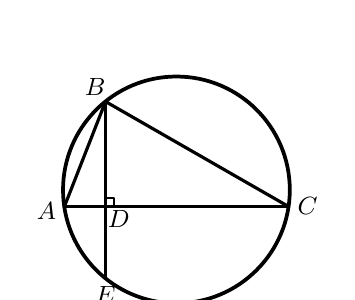
\begin{tikzpicture}[scale=0.60,line cap=round,line join=round]
  \coordinate (O) at (0,0);
  \coordinate (A) at (-2.37,-0.35);
  \coordinate (B) at (-1.50,1.87);
  \coordinate (C) at (2.37,-0.35);
  \coordinate (E) at (-1.50,-1.87);
  \coordinate (D) at (-1.50,-0.35);
  \draw[line width=1.35pt] (O) circle (2.40);
  \draw[line width=1.15pt] (A)--(C);
  \draw[line width=1.15pt] (B)--(E);
  \draw[line width=1.15pt] (A)--(B)--(C);
  \draw[line width=0.8pt] ($(D)+(0,0)$)--($(D)+(0,0.18)$)--($(D)+(0.18,0.18)$)--($(D)+(0.18,0)$);
  \node[font=\small\bfseries] at (-2.75,-0.45) {\(A\)};
  \node[font=\small\bfseries] at (-1.72,2.18) {\(B\)};
  \node[font=\small\bfseries] at (2.78,-0.35) {\(C\)};
  \node[font=\small\bfseries] at (-1.50,-2.23) {\(E\)};
  \node[font=\small\bfseries] at (-1.22,-0.62) {\(D\)};
\end{tikzpicture}%
}

\begin{document}

\begin{center}
  {\Large\bfseries Novel Prep Learning Center}\\[0.12cm]
  {\LARGE\bfseries\textcolor{npDeep}{Upper Math Placement Test}}\\[0.12cm]
  {\large Five-Gate Hybrid Diagnostic: Algebra I through Calculus Readiness}\\[0.45cm]
  Name:\ \ansline \hfill Date:\ \ansline
\end{center}

\begin{titlebox}
\textbf{Directions.} Choose the best answer for each question. Calculators should not be used unless the instructor specifically permits them. This diagnostic is designed to identify the best starting point among Algebra I, Geometry, Algebra II, Precalculus, and Calculus-readiness coursework.
\end{titlebox}

\begin{guidebox}
\textbf{Teacher Use.} This hybrid version combines the strongest items from the original upper-math placement set with a clearer five-gate diagnostic structure. Each gate contains 16 questions. A student should normally pass the current gate before being placed into the next course level. The total score is useful, but the gate pattern is more important than the total alone.
\end{guidebox}

\sectiontag{Gate 1: Algebra I Readiness}
\begin{enumerate}[leftmargin=0pt,itemindent=0pt,labelsep=0.55em,align=left]

\q{1} A factor of \(x^2-8x+15\) is
\mc{\(x-3\)}{\(x+3\)}{\(x+5\)}{\(x-8\)}{\(x-15\)}

\q{2} One solution to \(2x^2-5x-3=0\) is
\mc{\(-3\)}{\(-1\)}{\(0\)}{\(1\)}{\(3\)}

\q{3} \(\displaystyle \frac{t^2+7t+12}{t+3}=\)
\mc{\(t+3\)}{\(t+4\)}{\(t+7\)}{\(t^2+4\)}{\(t^2+7\)}

\q{4} One solution to \(x^2+2x-15=0\) is
\mc{\(-3\)}{\(-1\)}{\(1\)}{\(2\)}{\(3\)}

\q{5} If \(x=-2\) and \(y=3\), then \(\displaystyle \frac{x^2+xy}{x^2-y}=\)
\mc{\(-2\)}{\(-1\)}{\(0\)}{\(1\)}{\(2\)}

\q{6} If \(\displaystyle \frac{5}{x-1}=\frac{2}{x+2}\), then \(x=\)
\mc{\(-6\)}{\(-4\)}{\(-2\)}{\(2\)}{\(4\)}

\q{7} \(\displaystyle \frac{a}{b}+\frac{b-a}{b}=\)
\mc{\(0\)}{\(\dfrac{a}{b}\)}{\(1\)}{\(\dfrac{b-a}{b}\)}{\(\dfrac{2a-b}{b}\)}

\q{8} The line through \((1,2)\) and \((5,-2)\) has equation
\mc{\(y=-x+3\)}{\(y=x+1\)}{\(y=-x-1\)}{\(y=\dfrac12x+\dfrac32\)}{\(y=-2x+4\)}

\q{9} The \(x\)-intercept of \(y=4x-20\) is
\mc{\(-5\)}{\(0\)}{\(4\)}{\(5\)}{\(20\)}

\q{10} For the solution to
\[
\begin{cases}
2x+3y=13\\
x-y=1
\end{cases}
\]
the value of \(y\) is
\mc{\(1\)}{\(\dfrac{3}{2}\)}{\(2\)}{\(\dfrac{9}{5}\)}{\(\dfrac{11}{5}\)}

\q{11} The line passing through \((-1,4)\) and parallel to \(y=-3x+2\) is
\mc{\(y=-3x+4\)}{\(y=3x+1\)}{\(y=-3x+1\)}{\(y=-x+3\)}{\(y=3x-1\)}

\q{12} \((3x-y)(3x+y)=\)
\mc{\(9x^2+y^2\)}{\(9x^2-y^2\)}{\(6x^2-y^2\)}{\(9x^2-6xy-y^2\)}{\(9x^2+6xy-y^2\)}

\q{13} If \(3x+7=16\), then \(2x-1=\)
\mc{\(3\)}{\(4\)}{\(5\)}{\(6\)}{\(7\)}

\q{14} \(12ab^2-18a^2b+6ab=\)
\mc{\(6ab(2b-3a+1)\)}{\(6ab(2b-3a-1)\)}{\(6a(2b-3a+1)\)}{\(6b(2b-3a+1)\)}{\(12ab(b-a)+6ab\)}

\q{15} \((2x^2-x+5)-(x^2+4x-3)=\)
\mc{\(x^2-5x+8\)}{\(x^2+3x+2\)}{\(x^2-3x+8\)}{\(-x^2-5x+8\)}{\(x^2-5x-8\)}

\q{16} \((\sqrt{a}-3)^2=\)
\mc{\(a-3\sqrt a+9\)}{\(a-6\sqrt a+9\)}{\(a+6\sqrt a+9\)}{\(a-6\sqrt a-9\)}{\(a+9\)}

\newpage
\sectiontag{Gate 2: Geometry Readiness}

\q{17} A regular tetrahedron has all six edges equal to \(96\) cm. If its total surface area is \(k\sqrt3\) square centimeters, what is \(k\)?
\mc{\(9216\)}{\(4608\)}{\(18432\)}{\(2304\)}{\(27648\)}

\q{18} A square right pyramid has volume \(400\) cubic inches and slant height \(13\) inches. Its base side length and height are positive integers. What is its surface area in square inches?
\mc{\(320\)}{\(360\)}{\(400\)}{\(440\)}{\(480\)}

\q{19} A composite solid is formed by attaching a hemisphere of radius \(3\) to one circular base of a cylinder and a cone of height \(4\) to the other circular base. The cylinder has radius \(3\) and height \(10\). What is the total volume of the solid?
\mc{\(102\pi\)}{\(108\pi\)}{\(120\pi\)}{\(126\pi\)}{\(132\pi\)}

\q{20} A right circular cone has radius \(9\) and height \(12\). A smaller cone is removed from the top by a plane parallel to the base, \(4\) units from the vertex. What is the volume of the remaining frustum?
\mc{\(216\pi\)}{\(252\pi\)}{\(288\pi\)}{\(312\pi\)}{\(324\pi\)}

\needspace{9\baselineskip}
\q{21} Two similar triangles have side-length ratio \(1:3\). If the area of the smaller triangle is \(8\), what is the area of the larger triangle?
\mc{\(24\)}{\(36\)}{\(48\)}{\(72\)}{\(96\)}

\q{22} Rectangular prism A and rectangular prism B are similar. The height of prism A is \(4\) inches and the height of prism B is \(10\) inches. If the volume of prism A is \(200\) cubic inches, what is the volume of prism B?
\mc{\(1250\)}{\(2500\)}{\(3125\)}{\(5000\)}{\(6125\)}

\q{23} The distance between \((1,-2)\) and \((5,1)\) is
\mc{\(4\)}{\(5\)}{\(\sqrt7\)}{\(\sqrt{17}\)}{\(7\)}

\q{24} The equation of the circle with center \((2,-1)\) and radius \(4\) is
\mc{\((x+2)^2+(y-1)^2=16\)}{\((x-2)^2+(y+1)^2=16\)}{\((x-2)^2+(y-1)^2=16\)}{\((x+2)^2+(y+1)^2=16\)}{\(x^2+y^2=16\)}

\q{25} Quadrilateral \(ABCD\) has vertices
\[
A(-2,1),\quad B(3,3),\quad C(5,-2),\quad D(0,-4).
\]
Which classification is most specific?
\mc{rectangle}{rhombus}{square}{parallelogram only}{trapezoid}

\q{26} Triangle \(ABC\) has vertices \(A(-3,2)\), \(B(-1,6)\), and \(C(2,3)\). It is reflected across the \(y\)-axis and then translated \(4\) units down. What are the coordinates of \(A'B'C'\)?
\mc{\((-3,-2),(-1,2),(2,-1)\)}{\((3,-2),(1,2),(-2,-1)\)}{\((3,6),(1,10),(-2,7)\)}{\((-3,6),(-1,10),(2,7)\)}{\((2,-3),(6,-1),(3,2)\)}

\needspace{18\baselineskip}
\q{27} In the figure shown, points \(A\), \(B\), \(C\), and \(E\) lie on the circle, and \(AB<BC\). Segment \(AC\) is perpendicular to segment \(BE\) at point \(D\), and \(BD=\sqrt{346}\). The diameter of the circle is \(175\). If \(\dfrac{CD}{AD}=r\), what is the value of \(r\) (\(\angle ABC\) is a right angle)?

\begin{center}
\circleChordDiagram
\end{center}

\mc{\(86.5\)}{\(85.5\)}{\(90\)}{\(216\)}{\(324\)}

\q{28} In \(\triangle ABC\), \(m\angle A=45^\circ\), \(m\angle B=75^\circ\), and side \(a=8\sqrt2\). Using standard notation, what is the exact value of side \(b\)?
\mc{\(8(\sqrt3+1)\)}{\(4(\sqrt6+\sqrt2)\)}{\(8\sqrt3\)}{\(12\sqrt2\)}{\(16\)}

\q{29} In a right triangle, the altitude to the hypotenuse divides the hypotenuse into segments of lengths \(9\) and \(16\). What is the length of the altitude?
\mc{\(10\)}{\(11\)}{\(12\)}{\(13\)}{\(15\)}

\q{30} In the \(xy\)-plane, the graph of \(x^2+6x+y^2+2y=15\) is a circle. Line \(k\) has a slope of \(\frac34\) and is tangent to this circle at the point \((a,b)\), where \(b\) is negative. What is the value of \(b\)?
\mc{\(-5\)}{\(-4\)}{\(-3\)}{\(-2\)}{\(-1\)}

\needspace{16\baselineskip}
\q{31} In right triangle \(\triangle ABC\), \(\angle B=90^\circ\), \(\overline{AB}=12\), and point \(D\) lies on \(\overline{AC}\). Segment \(\overline{BD}\) is drawn. Which of the following must be true?
\[
\begin{array}{ll}
\text{I.} & \overline{BC}=12\tan(\angle CAB)\\[0.25em]
\text{II.} & \cos(\angle ABD)-\sin(\angle DBC)=0\\[0.25em]
\text{III.} & \angle ABD=\angle BDC
\end{array}
\]
\mc{I and II only}{II and III only}{I and III only}{I, II, and III}{None}

\needspace{6\baselineskip}
\item[\circnum{32}] A triangle has sides of length \(9\) and \(14\), and the included angle between them is \(120^\circ\). What is the square of the third side?
\mc{\(151\)}{\(277\)}{\(322\)}{\(403\)}{\(529\)}

\sectiontag{Gate 2 Extension: Counting, Probability, and Conics}

\q{33} How many committees of \(6\) people can be chosen from \(11\) people? If the same \(6\) people are taking \(6\) different positions on the committee, how many assignments are possible?
\mc{\(462;\ 332{,}640\)}{\(462;\ 720\)}{\(66;\ 332{,}640\)}{\(332{,}640;\ 462\)}{\(11^6;\ 6!\)}

\q{34} A bowl contains \(6\) red marbles and \(3\) blue marbles. Three marbles are drawn at random, one after another, without replacement. What is the probability of getting a red marble first, then a blue marble, then a red marble?
\mc{\(\dfrac{1}{7}\)}{\(\dfrac{5}{28}\)}{\(\dfrac{2}{9}\)}{\(\dfrac{5}{14}\)}{\(\dfrac{1}{3}\)}

\q{35} A statistics class has \(8\) seniors, \(6\) juniors, \(13\) sophomores, and \(3\) freshmen. A class committee must have \(1\) senior, \(2\) juniors, \(3\) sophomores, and \(1\) freshman. How many such committees are possible?
\mc{\(17{,}160\)}{\(34{,}320\)}{\(102{,}960\)}{\(205{,}920\)}{\(1{,}029{,}600\)}

\q{36} Write the equation of the ellipse with center \((2,-3)\), one focus \((5,-3)\), and one vertex \((6,-3)\).
\mc{\(\dfrac{(x-2)^2}{7}+\dfrac{(y+3)^2}{16}=1\)}{\(\dfrac{(x+2)^2}{16}+\dfrac{(y-3)^2}{7}=1\)}{\(\dfrac{(x-2)^2}{16}+\dfrac{(y+3)^2}{9}=1\)}{\(\dfrac{(x-2)^2}{16}+\dfrac{(y+3)^2}{7}=1\)}{\(\dfrac{(x-2)^2}{4}+\dfrac{(y+3)^2}{3}=1\)}

\q{37} Write the equation of a parabola with vertex \((2,-8)\) and directrix \(x=3\).
\mc{\((y+8)^2=-4(x-2)\)}{\((y+8)^2=4(x-2)\)}{\((x-2)^2=-4(y+8)\)}{\((x-2)^2=4(y+8)\)}{\((y-8)^2=-4(x+2)\)}

\newpage
\sectiontag{Gate 3: Algebra II Readiness}

\q{38} Solve \(x^2-5x-14=0\).
\mc{\(x=2,-7\)}{\(x=-7,-2\)}{\(x=7,-2\)}{\(x=14,-1\)}{\(x=5,-14\)}

\q{39} The discriminant of \(2x^2+4x+5=0\) indicates
\mc{two real rational solutions}{one real solution}{two real irrational solutions}{two non-real complex solutions}{infinitely many solutions}

\q{40} Simplify \(\sqrt{75x^4}\), assuming \(x\) is real.
\mc{\(5x^2\sqrt3\)}{\(25x^2\sqrt3\)}{\(5x\sqrt3\)}{\(75x^2\)}{\(3x^2\sqrt5\)}

\q{41} Simplify \((3+2i)(4-i)\).
\mc{\(10+5i\)}{\(14+5i\)}{\(14+11i\)}{\(12-2i\)}{\(10-5i\)}

\q{42} Evaluate \(27^{2/3}\).
\mc{\(3\)}{\(6\)}{\(9\)}{\(18\)}{\(81\)}

\q{43} Solve \(\sqrt{x+5}=x-1\).
\mc{\(x=1\)}{\(x=2\)}{\(x=-1\)}{\(x=4\)}{no solution}

\q{44} The vertex of \(y=(x-3)^2-7\) is
\mc{\((-3,-7)\)}{\((3,-7)\)}{\((-3,7)\)}{\((3,7)\)}{\((0,-7)\)}

\q{45} Factor \(2x^2-7x-15\).
\mc{\((2x+3)(x-5)\)}{\((2x-3)(x+5)\)}{\((x+3)(2x-5)\)}{\((2x-5)(x+3)\)}{prime}

\q{46} If \(f(x)=2x-1\) and \(g(x)=x^2+3\), then \(f(g(2))=\)
\mc{\(7\)}{\(10\)}{\(13\)}{\(15\)}{\(17\)}

\q{47} The average rate of change of \(f(x)=x^2\) on \([1,4]\) is
\mc{\(3\)}{\(5\)}{\(6\)}{\(8\)}{\(15\)}

\q{48} \(\log_2 32=\)
\mc{\(5\)}{\(8\)}{\(16\)}{\(30\)}{\(64\)}

\q{49} The model \(P(t)=400(1.08)^t\) represents a quantity that
\mc{starts at 1.08}{decreases by 8 percent}{grows by 8 percent}{grows by 400 percent}{doubles every 8 years}

\q{50} Solve \(3^{x+1}=27\).
\mc{\(x=0\)}{\(x=1\)}{\(x=3\)}{\(x=2\)}{\(x=4\)}

\q{51} Simplify \(\dfrac{x^2-4}{x+2}\), where \(x\neq -2\).
\mc{\(x+2\)}{\(x-2\)}{\(x^2-2\)}{\(x^2+2\)}{\(1\)}

\q{52} The remainder when \(x^3-3x+1\) is divided by \(x-2\) is
\mc{\(-3\)}{\(-1\)}{\(0\)}{\(1\)}{\(3\)}

\q{53} If \(f(x)=\dfrac{x-5}{3}\), then \(f^{-1}(x)=\)
\mc{\(\dfrac{x+5}{3}\)}{\(\dfrac{x-3}{5}\)}{\(3x-5\)}{\(3x+5\)}{\(\dfrac{3}{x-5}\)}

\newpage
\sectiontag{Gate 4: Precalculus Readiness}

\q{54} \(\sin 210^\circ=\)
\mc{\(\frac12\)}{\(-\frac12\)}{\(\frac{\sqrt3}{2}\)}{\(-\frac{\sqrt3}{2}\)}{\(0\)}

\q{55} If \(\tan\theta=\frac34\) and \(\theta\) is in Quadrant I, then \(\cos\theta=\)
\mc{\(\frac35\)}{\(\frac34\)}{\(\frac45\)}{\(\frac43\)}{\(\frac53\)}

\q{56} Which function has amplitude 4 and period \(\pi\)?
\mc{\(y=4\sin 2x\)}{\(y=2\sin 4x\)}{\(y=4\sin x\)}{\(y=\sin 4x\)}{\(y=4\cos\frac{x}{2}\)}

\q{57} Which expression is equal to \(\cos 2x\)?
\mc{\(2\cos^2x-1\)}{\(1-2\sin^2x\)}{\(\cos^2x-\sin^2x\)}{none of A, B, and C}{A, B, and C}

\q{58} If \(\ln w=\ln a+\ln b-\ln c\), then \(w=\)
\mc{\(a+b-c\)}{\(\dfrac{ab}{c}\)}{\(abc\)}{\(\dfrac{ac}{b}\)}{\(\dfrac{c}{ab}\)}

\q{59} The domain of \(f(x)=\dfrac{\sqrt{x-2}}{x+1}\) is
\mc{\([2,\infty)\)}{\((-1,\infty)\)}{\([2,\infty)\setminus\{-1\}\)}{\((-\infty,-1)\cup(-1,\infty)\)}{\((2,\infty)\)}

\q{60} If \(f(x)=2x+7\), then \(f^{-1}(x)=\)
\mc{\(\dfrac{x+7}{2}\)}{\(2x-7\)}{\(\dfrac{x-7}{2}\)}{\(7x+2\)}{\(\dfrac{2}{x-7}\)}

\q{61} The point on the unit circle corresponding to \(\frac{7\pi}{6}\) is
\mc{\(\left(\frac{\sqrt3}{2},\frac12\right)\)}{\(\left(-\frac12,-\frac{\sqrt3}{2}\right)\)}{\(\left(-\frac{\sqrt3}{2},\frac12\right)\)}{\(\left(-\frac{\sqrt3}{2},-\frac12\right)\)}{\(\left(\frac12,-\frac{\sqrt3}{2}\right)\)}

\q{62} Solve \(2\sin x=1\) on \([0,2\pi)\).
\mc{\(\frac{\pi}{6},\frac{5\pi}{6}\)}{\(\frac{\pi}{6},\frac{11\pi}{6}\)}{\(\frac{\pi}{3},\frac{2\pi}{3}\)}{\(\frac{5\pi}{6},\frac{11\pi}{6}\)}{\(\frac{7\pi}{6},\frac{11\pi}{6}\)}

\q{63} A triangle has sides \(7\) and \(10\) with included angle \(60^\circ\). By the Law of Cosines, the square of the third side is
\mc{\(49\)}{\(79\)}{\(119\)}{\(149\)}{\(249\)}

\q{64} Convert \(150^\circ\) to radians.
\mc{\(\frac{2\pi}{3}\)}{\(\frac{3\pi}{4}\)}{\(\frac{5\pi}{6}\)}{\(\frac{7\pi}{6}\)}{\(\frac{5\pi}{4}\)}

\q{65} A sector has radius 5 and central angle \(\frac{4\pi}{5}\). Its arc length is
\mc{\(2\pi\)}{\(3\pi\)}{\(5\pi\)}{\(4\pi\)}{\(10\pi\)}

\q{66} The graph of \(y=\log_2(x-3)+1\) has vertical asymptote
\mc{\(x=-3\)}{\(x=3\)}{\(x=1\)}{\(y=1\)}{\(y=3\)}

\q{67} The horizontal asymptote of \(y=\dfrac{2x^2+1}{x^2-4}\) is
\mc{\(y=2\)}{\(y=1\)}{\(y=-4\)}{\(x=2\)}{none}

\q{68} Solve \(\log_3(x-1)=2\).
\mc{\(x=3\)}{\(x=4\)}{\(x=8\)}{\(x=9\)}{\(x=10\)}

\q{69} The model \(A(t)=1200(0.92)^t\) represents a quantity that
\mc{starts at \(0.92\)}{grows by \(92\%\)}{decreases by \(8\%\)}{decreases by \(92\%\)}{starts at \(8\)}

\newpage
\sectiontag{Gate 5: Calculus Readiness}

\q{70} Evaluate \(\displaystyle \lim_{x\to3}\frac{x^2-9}{x-3}\).
\mc{\(0\)}{\(6\)}{\(9\)}{\(3\)}{does not exist}

\q{71} If \(f(x)=3x^2-5x+1\), then \(f'(x)=\)
\mc{\(3x-5\)}{\(6x+5\)}{\(6x-5\)}{\(x^3-\frac52x^2+x\)}{\(3x^2-5\)}

\q{72} The slope of the tangent line to \(y=x^2\) at \(x=-2\) is
\mc{\(-4\)}{\(-2\)}{\(0\)}{\(2\)}{\(4\)}

\q{73} The average rate of change of \(f(x)=x^2+1\) on \([1,4]\) is
\mc{\(3\)}{\(5\)}{\(6\)}{\(8\)}{\(15\)}

\q{74} Evaluate \(\displaystyle \lim_{x\to0}\frac{\sin x}{x}\).
\mc{\(0\)}{\(-1\)}{\(\infty\)}{\(1\)}{does not exist}

\q{75} If \(f(x)=e^x+\ln x\), then \(f'(x)=\)
\mc{\(e^x+\ln x\)}{\(e^x+x\)}{\(e^x-\frac1x\)}{\(xe^x\)}{\(e^x+\frac1x\)}

\q{76} \(\dfrac{d}{dx}(\sin x)=\)
\mc{\(\cos x\)}{\(-\cos x\)}{\(\tan x\)}{\(-\sin x\)}{\(\sec^2x\)}

\q{77} If \(f(x)=x^3-4x\), then \(f'(2)=\)
\mc{\(4\)}{\(6\)}{\(8\)}{\(10\)}{\(12\)}

\q{78} Let
\[
f(x)=
\begin{cases}
x+2, & x<1,\\
ax, & x\ge 1.
\end{cases}
\]
For \(f\) to be continuous at \(x=1\), \(a=\)
\mc{\(0\)}{\(1\)}{\(2\)}{\(-3\)}{\(3\)}

\q{79} If \(f'(x)\) changes from positive to negative at \(x=c\), then \(f\) has
\mc{a local minimum at \(c\)}{a local maximum at \(c\)}{a vertical asymptote at \(c\)}{no change at \(c\)}{a removable discontinuity at \(c\)}

\q{80} Evaluate \(\displaystyle \int_0^3 2x\,dx\).
\mc{\(3\)}{\(6\)}{\(8\)}{\(9\)}{\(18\)}

\q{81} A particle moves with constant velocity \(v(t)=5\) ft/s for \(0\le t\le4\). The distance traveled is
\mc{\(5\) ft}{\(10\) ft}{\(20\) ft}{\(25\) ft}{\(40\) ft}

\q{82} \(\dfrac{d}{dx}\left(x^2\sin x\right)=\)
\mc{\(2x\sin x+x^2\cos x\)}{\(x^2\cos x\)}{\(2x\cos x+x^2\sin x\)}{\(2x\sin x\)}{\(2x+\cos x\)}

\q{83} If \(f(x)=x^4\), then \(f''(x)=\)
\mc{\(4x^3\)}{\(12x^2\)}{\(24x\)}{\(x^2\)}{\(4x^2\)}

\q{84} The tangent line to \(y=x^2+1\) at \(x=1\) is
\mc{\(y=x+1\)}{\(y=2x+1\)}{\(y=2x\)}{\(y=x+2\)}{\(y=3x-1\)}

\q{85} Evaluate \(\displaystyle \lim_{x\to\infty}\frac{5x^2-1}{2x^2+3}\).
\mc{\(0\)}{\(1\)}{\(2\)}{\(\frac52\)}{\(\infty\)}

\end{enumerate}

\newpage
\section*{Student Answer Grid}
\begin{titlebox}
\textbf{Directions.} Fill in exactly one answer for each question. Erase clearly if you change an answer.
\end{titlebox}

\begin{center}
\scriptsize
\setlength{\tabcolsep}{3pt}
\begin{tabular}{p{0.30\textwidth}p{0.30\textwidth}p{0.30\textwidth}}
\answerrow{1} & \answerrow{30} & \answerrow{59}\\
\answerrow{2} & \answerrow{31} & \answerrow{60}\\
\answerrow{3} & \answerrow{32} & \answerrow{61}\\
\answerrow{4} & \answerrow{33} & \answerrow{62}\\
\answerrow{5} & \answerrow{34} & \answerrow{63}\\
\answerrow{6} & \answerrow{35} & \answerrow{64}\\
\answerrow{7} & \answerrow{36} & \answerrow{65}\\
\answerrow{8} & \answerrow{37} & \answerrow{66}\\
\answerrow{9} & \answerrow{38} & \answerrow{67}\\
\answerrow{10} & \answerrow{39} & \answerrow{68}\\
\answerrow{11} & \answerrow{40} & \answerrow{69}\\
\answerrow{12} & \answerrow{41} & \answerrow{70}\\
\answerrow{13} & \answerrow{42} & \answerrow{71}\\
\answerrow{14} & \answerrow{43} & \answerrow{72}\\
\answerrow{15} & \answerrow{44} & \answerrow{73}\\
\answerrow{16} & \answerrow{45} & \answerrow{74}\\
\answerrow{17} & \answerrow{46} & \answerrow{75}\\
\answerrow{18} & \answerrow{47} & \answerrow{76}\\
\answerrow{19} & \answerrow{48} & \answerrow{77}\\
\answerrow{20} & \answerrow{49} & \answerrow{78}\\
\answerrow{21} & \answerrow{50} & \answerrow{79}\\
\answerrow{22} & \answerrow{51} & \answerrow{80}\\
\answerrow{23} & \answerrow{52} & \answerrow{81}\\
\answerrow{24} & \answerrow{53} & \answerrow{82}\\
\answerrow{25} & \answerrow{54} & \answerrow{83}\\
\answerrow{26} & \answerrow{55} & \answerrow{84}\\
\answerrow{27} & \answerrow{56} & \answerrow{85}\\
\answerrow{28} & \answerrow{57} & \\
\answerrow{29} & \answerrow{58} & \\
\end{tabular}
\end{center}

\newpage
\section*{Teacher Scoring Guide}

\begin{guidebox}
\textbf{Gate scores.} Gate 1 and Gates 3--5 each contain 16 questions. Gate 2 contains 21 questions because it includes an advanced geometry extension with counting, probability, and conics. Use gate scores first and total score second. A high total score should not override a weak prerequisite gate.
\end{guidebox}

\begin{center}
\begin{tabularx}{\linewidth}{>{\bfseries}p{0.22\linewidth}p{0.18\linewidth}X}
\toprule
Gate & Items & Primary Meaning\\
\midrule
Gate 1 & Q1--16 & Algebra I readiness: equations, functions, linear models, factoring, systems, and symbolic fluency.\\
Gate 2 & Q17--37 & Geometry readiness plus extension: composite solids, similarity, coordinate geometry, transformations, circles, right-triangle reasoning, Law of Sines, Law of Cosines, counting, probability, and conics.\\
Gate 3 & Q38--53 & Algebra II readiness: quadratics, complex numbers, radicals, rational expressions, exponentials, logs, and composition.\\
Gate 4 & Q54--69 & Precalculus readiness: trigonometry, unit circle, logs, inverse functions, rational behavior, and advanced function analysis.\\
Gate 5 & Q70--85 & Calculus readiness: limits, derivative fluency, continuity, tangent slope, average rate of change, and basic integral meaning.\\
\bottomrule
\end{tabularx}
\end{center}

\begin{titlebox}
\textbf{Suggested placement rules.}
\begin{itemize}[leftmargin=1.3em,itemsep=0.22em]
\item \textbf{Algebra I:} Gate 1 below 11/16, or major arithmetic/algebra instability.
\item \textbf{Geometry:} Gate 1 at least 11/16 and Gate 2 below 13/21.
\item \textbf{Algebra II:} Gate 1 at least 11/16, Gate 2 at least 13/21, and Gate 3 below 11/16.
\item \textbf{Precalculus:} Gate 1 at least 11/16, Gate 2 at least 13/21, Gate 3 at least 11/16, and Gate 4 below 12/16.
\item \textbf{Calculus-ready:} Gate 1 at least 12/16, Gate 2 at least 16/21, Gates 3--4 at least 12/16, and Gate 5 at least 11/16.
\end{itemize}
\end{titlebox}

\begin{guidebox}
\textbf{Gate 2 interpretation.} Use \(13/21\) as standard geometry readiness and \(16/21\) or higher as strong geometry/enhanced readiness. A student who scores \(13\)--\(15\) but misses most of Q19, Q20, Q27, Q28, Q30, and Q32--37 should receive targeted review before Algebra II or Precalculus placement.
\end{guidebox}

\begin{guidebox}
\textbf{Score Card}
\[
\begin{array}{c|ccccc|c}
\text{Gate} & 1 & 2 & 3 & 4 & 5 & \text{Total}\\ \hline
\text{Items} & 1\text{--}16 & 17\text{--}37 & 38\text{--}53 & 54\text{--}69 & 70\text{--}85 & 85\\
\text{Correct} & \rule{0.5in}{0.4pt} & \rule{0.5in}{0.4pt} & \rule{0.5in}{0.4pt} & \rule{0.5in}{0.4pt} & \rule{0.5in}{0.4pt} & \rule{0.65in}{0.4pt}
\end{array}
\]
\end{guidebox}

\newpage
\section*{Study Plan by Placement Band}

\begin{center}
\begin{tabularx}{\linewidth}{>{\bfseries}p{0.18\linewidth}p{0.16\linewidth}X}
\toprule
Placement Band & Suggested Plan & Focus\\
\midrule
Algebra I support & 20--30 lessons & Equations, inequalities, linear graphs, function notation, factoring foundations, systems, and word-problem translation.\\
Geometry bridge & 12--20 lessons & Algebra review plus angle relationships, triangle congruence, similarity, coordinate geometry, transformations, circles, composite solids, Law of Sines/Cosines, counting/probability, and conics.\\
Algebra II bridge & 16--24 lessons & Quadratics, radicals, rational expressions, complex numbers, exponentials/logs, composition, and modeling.\\
Precalculus bridge & 18--26 lessons & Trigonometry, unit circle, identities, inverse functions, rational functions, logs, conics, and advanced graph analysis.\\
Calculus bridge & 8--14 lessons & Limit notation, continuity, derivative meaning, tangent slope, rate of change, derivative rules, and area/accumulation concepts.\\
\bottomrule
\end{tabularx}
\end{center}

\newpage
\section*{Answer Key}

\begin{multicols}{4}
\begin{enumerate}[leftmargin=1.8em,itemsep=0.12em,label=\textbf{\arabic*.}]
\item A
\item E
\item B
\item E
\item A
\item B
\item C
\item A
\item D
\item E
\item C
\item B
\item C
\item A
\item A
\item B
\item A
\item B
\item C
\item D
\item D
\item C
\item B
\item B
\item C
\item B
\item A
\item B
\item C
\item A
\item A
\item D
\item B
\item B
\item C
\item D
\item A
\item C
\item D
\item A
\item B
\item C
\item D
\item B
\item A
\item C
\item B
\item A
\item C
\item D
\item B
\item E
\item D
\item B
\item C
\item A
\item E
\item B
\item A
\item C
\item D
\item A
\item B
\item C
\item D
\item B
\item A
\item E
\item C
\item B
\item C
\item A
\item B
\item D
\item E
\item A
\item C
\item E
\item B
\item D
\item C
\item A
\item B
\item C
\item D
\end{enumerate}
\end{multicols}

\end{document}
